
\documentclass[notheorems,serif,table,compress]{beamer}  %dvipdfm选项是关键,否则编译统统通不过
%%------------------------常用宏包------------------------
%%注意, beamer 会默认使用下列宏包: amsthm, graphicx, hyperref, color, xcolor, 等等
\usepackage{fontspec,xunicode,xltxtra}  % for XeTeX
\usepackage{verbatim}
\usepackage{mathabx}
\usepackage{latexsym}
\usepackage{amsfonts,amssymb}
\usepackage{styles/iplouclistings}
\usepackage{fancybox}
\usepackage{colortbl}
\usepackage{tcolorbox}
%\usepackage[T1]{fontenc}
%\usepackage{bookman}
\usepackage{subfigure}
\usepackage{hyperref}
\usepackage{listings}
\usepackage{animate}
\usepackage[absolute,overlay]{textpos}
\usepackage{graphicx}
\usepackage{tikz}
\usepackage[americaninductors,europeanresistors]{circuitikz}
\usepackage{tikz}
\usepackage{fancybox}     %% 定义zhushadow时用到
\usepackage{pifont} %ding用到
\newsavebox{\mysaveboxOne}  %%为了在only中使用lstlisting
\newsavebox{\mysaveboxTwo}
\newsavebox{\mysaveboxThree}
\newsavebox{\mysaveboxFour}
\newsavebox{\mysaveboxFive}
\newsavebox{\mysaveboxSix}
\newsavebox{\mysaveboxSeven}
\newcommand\zhushadow[2][purple]{\hskip5pt\shadowbox{\color{#1}\small\kai #2\vspace{3mm}}}

%%------------------------ThemeColorFont------------------------
%% Presentation Themes
% \usetheme[<options>]{<name list>}
%\usetheme{Madrid}
\usetheme{Berkeley}
%% Inner Themes双精度计算
% \useinnertheme[<options>]{<name>}
%% Outer Themes
% \useoutertheme[<options>]{<name>}
%\useoutertheme{miniframes} 
%% Color Themes 
%\usecolortheme[<options>]{<name list>}
%% Font Themes
\usefonttheme{serif}
\setbeamertemplate{background canvas}[vertical shading][bottom=white,top=structure.fg!7] %%背景色, 上25%的蓝, 过渡到下白.
\setbeamertemplate{theorems}[numbered]
\setbeamertemplate{navigation symbols}{}   %% 去掉页面下方默认的导航条.
\usepackage{styles/zhfontcfg}
%\setsansfont[Mapping=tex-text]{文泉驿正黑}  %% 需要fontspec宏包
     %如果装了Adobe Acrobat,可在font.conf中配置Adobe字体的路径以使用其中文字体
     %也可直接使用系统中的中文字体如SimSun,SimHei,微软雅黑 等
     %原来beamer用的字体是sans family;注意Mapping的大小写,不能写错
     %设置字体时也可以直接用字体名,以下三种方式等同:
     %\setromanfont[BoldFont={黑体}]{宋体}
     %\setromanfont[BoldFont={SimHei}]{SimSun}
     %\setromanfont[BoldFont={"[simhei.ttf]"}]{"[simsun.ttc]"}
%%------------------------MISC------------------------
\graphicspath{{figures/}}         %% 图片路径. 本文的图片都放在这个文件夹里了.
%%------------------------listing------------------------
%\lstset{language=[LaTeX]TeX,Python}
%%------------------------正文------------------------
\begin{document}
\XeTeXlinebreaklocale "zh"         % 表示用中文的断行
\XeTeXlinebreakskip = 0pt plus 1pt % 多一点调整的空间
%%----------------------------------------------------------
%% This is only inserted into the PDF information catalog. Can be left
%% out.
%%%
%% Delete this, if you do not want the table of contents to pop up at
%% the beginning of each subsection:
%\AtBeginSection[]{                              % 在每个Section前都会加入的Frame
%  \frame<handout:0>{
%    \frametitle{Contents}\small
%    \tableofcontents[current,currentsubsection]
%  }
%}
%
%\AtBeginSubsection[]                            % 在每个子段落之前
%{
%  \frame<handout:0>                             % handout:0 表示只在手稿中出现
%  {
%    \frametitle{Contents}\small
%    \tableofcontents[current,currentsubsection] % 显示在目录中加亮的当前章节
%  }
%}

\setbeamertemplate{caption}{\raggedright\insertcaption\par}

%%----------------------------------------------------------
\logo{
\includegraphics[scale=0.13]{ouclogo.png}}
\title{Histograms of Oriented Gradients}
%\subtitle{Bottom-Up Saliency Detection Model Based on Human Visual Sensitivity and Amplitude Spectrum}
\subtitle{梯度方向直方图}
\author[]{\textcolor{olive}{TangNing}}
\institute[CVBIOUC]
{
\small\textcolor{violet}{CVBIOUC\\
%Ocean University of China\\
\url{http://vision.ouc.edu.cn/~zhenghaiyong}}
}
%\date[]{}
%\titlegraphic{
%
\includegraphics[height=1.0cm]{ouc-logo.jpg}}
\frame{ \titlepage }
%%----------------------------------------------------------
%\section*{Contents}
\frame{\frametitle{Contents}\tableofcontents}
%%----------------------------------------------------------
\def\hilite<#1>{\temporal<#1>{\color{blue!15}}{\color{black}}{\color{black}}}
\newcommand{\shadow}[2][purple]{\hskip5pt\shadowbox{\color{#1}\small \kai #2\vspace{3mm}}}
\newcommand{\colorrbox}[2][purple]{\doublebox{\color{#1}\small \kai#2}}

%============================================================================

\section{Brife Introduction}

%==========================================================================

\subsection{Main Thoughts}
\begin{frame}
\frametitle{Main Thoughts}
Histograms of Oriented Gradients (HOG) is a technique for feature extraction, which is extensively used in human detection:
    \begin{itemize}
        \item {\color{blue}Substance: }the statistics of gradient information in some dense overlapping grids.
        \item {\color{blue}Basic Idea: }local object appearance and shape can often be characterized rather well by the distribution of local intensity gradients edge directions.
    \end{itemize}
\end{frame}

%============================================================================

\section{Steps in HOG Feature Extraction}

%============================================================================
\subsection{The Flow Chart of HOG Feature Extraction}
\begin{frame}
\frametitle{The Flow Chart of HOG Feature Extraction}
\begin{figure}
    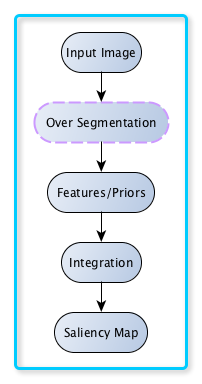
\includegraphics[width=0.6\linewidth]{flowchart.png} 
\end{figure}
\end{frame}
\subsection{The Detailed Process of HOG}
\begin{frame}
\frametitle{The Detailed Process of HOG}
\textbf{\color{blue}1. Gamma Normalization: } \\reduce the local shadow and illumination changes in image, yet it has a modest effect on performance because the subsequent normalization. (can be omitted)
\begin{displaymath}
I(x,y)=I(x,y)^{gamma}
\end{displaymath}
\begin{center}
for example, $gamma=\frac{1}{2}$
\end{center}
\end{frame}

\begin{frame}
\frametitle{The Detailed Process of HOG}
\textbf{\color{blue}2. Gradient Computation: }\\
capture the contour, human shadow, and texture information, weaken the effect of illumination. (Simple masks without Gaussian smoothing work best)\\
\begin{center}
{\textbf{Horizontal gradient operator: }} [-1, 0, 1] \\
{\textbf{Vertical gradient operator: }} [-1, 0, 1]$^{\rm T}$ 
\end{center}
The {\textbf{magnitude}} of the gradient:
    \begin{displaymath}
        M(x,y)=mag(\bigtriangledown f ~) = \sqrt{g_{x}^{2}+g_{y}^{2}}
    \end{displaymath}
The {\textbf{direction}} of the gradient:
    \begin{displaymath}
        \alpha (x,y)=arctan \left[ \frac{g_{x}}{g_{y}} \right]
    \end{displaymath}

\end{frame}


\begin{frame}        
\frametitle{Spatial / Orientation Binning}
\textbf{\color{blue}3. Spatial / Orientation Binning: }\\
each pixel calculates a weighted vote for an edge orientation histogram channel in the cell which belongs to. (For getting the best results: the orientation bins is $0^{\circ}$-$180^{\circ}$, the number of orientation bins is 9, the vote is magnitude)
\begin{figure}
    \includegraphics[width=0.4\linewidth]{cell.jpg}
    \includegraphics[width=0.5\linewidth]{bins.jpg}  
\end{figure}   
\end{frame}
\begin{frame}        
\frametitle{Spatial / Orientation Binning}
\begin{figure}
    \includegraphics[width=0.8\linewidth]{HOG.png} 
\end{figure}   
\end{frame}

\begin{frame}        
\frametitle{Normalization and Descriptor Blocks}
\textbf{\color{blue}4. Normalization and Descriptor Blocks: }\\
gradient strengths vary over a wide range owing to local variations in illumination and foreground-background contrast
\begin{itemize}
        \item grouping cells into larger spatial blocks. (Two arrangements: R-HOG, C-HOG)
\begin{figure}
    \includegraphics[width=0.6\linewidth]{block.jpg}
\end{figure}   
\end{itemize}
\end{frame}



\begin{frame}        
\frametitle{Normalization and Descriptor Blocks}
\begin{itemize}
        \item contrast normalizing each block separately. Let \textbf{\mathbf{v}} be the unnormalized descriptor vector, $\Vert \mathbf{v} \Vert_k$ be its $k-norm$ for $k$=1, 2, and
$\epsilon$ be a small constant.\\
\end{itemize}
\qquad{\color{blue}(a) $L2-norm$: } \textbf{\mathbf{v}}\to  \mathbf{v}/\sqrt{\Vert \mathbf{v} \Vert^{2}_2+\epsilon^{2}}\\
\qquad{\color{blue}(b) $L2-Hys$: } $L2-norm$ followed by clipping (limiting the maximum values of \mathbf{v} to 0.2) and renormalizing.\\
\qquad{\color{blue}(c) $L1-sqrt$: } \textbf{\mathbf{v}}\to  \sqrt{\mathbf{v}/(\vert \mathbf{v} \vert_1+\epsilon)}
\end{frame}

\begin{frame}        
\frametitle{Collect HOG Features for All Blocks}
\textbf{\color{blue}5. Collect HOG Features for All Blocks: }
\begin{figure}
    \includegraphics[width=0.6\linewidth]{block_cell.png}\\
    \includegraphics[width=0.6\linewidth]{HOG_vector.png}
\end{figure}   
\end{frame}
   
%===============================================================================


\end{document}
